% Created by tikzDevice version 0.12.6 on 2024-11-06 20:31:48
% !TEX encoding = UTF-8 Unicode
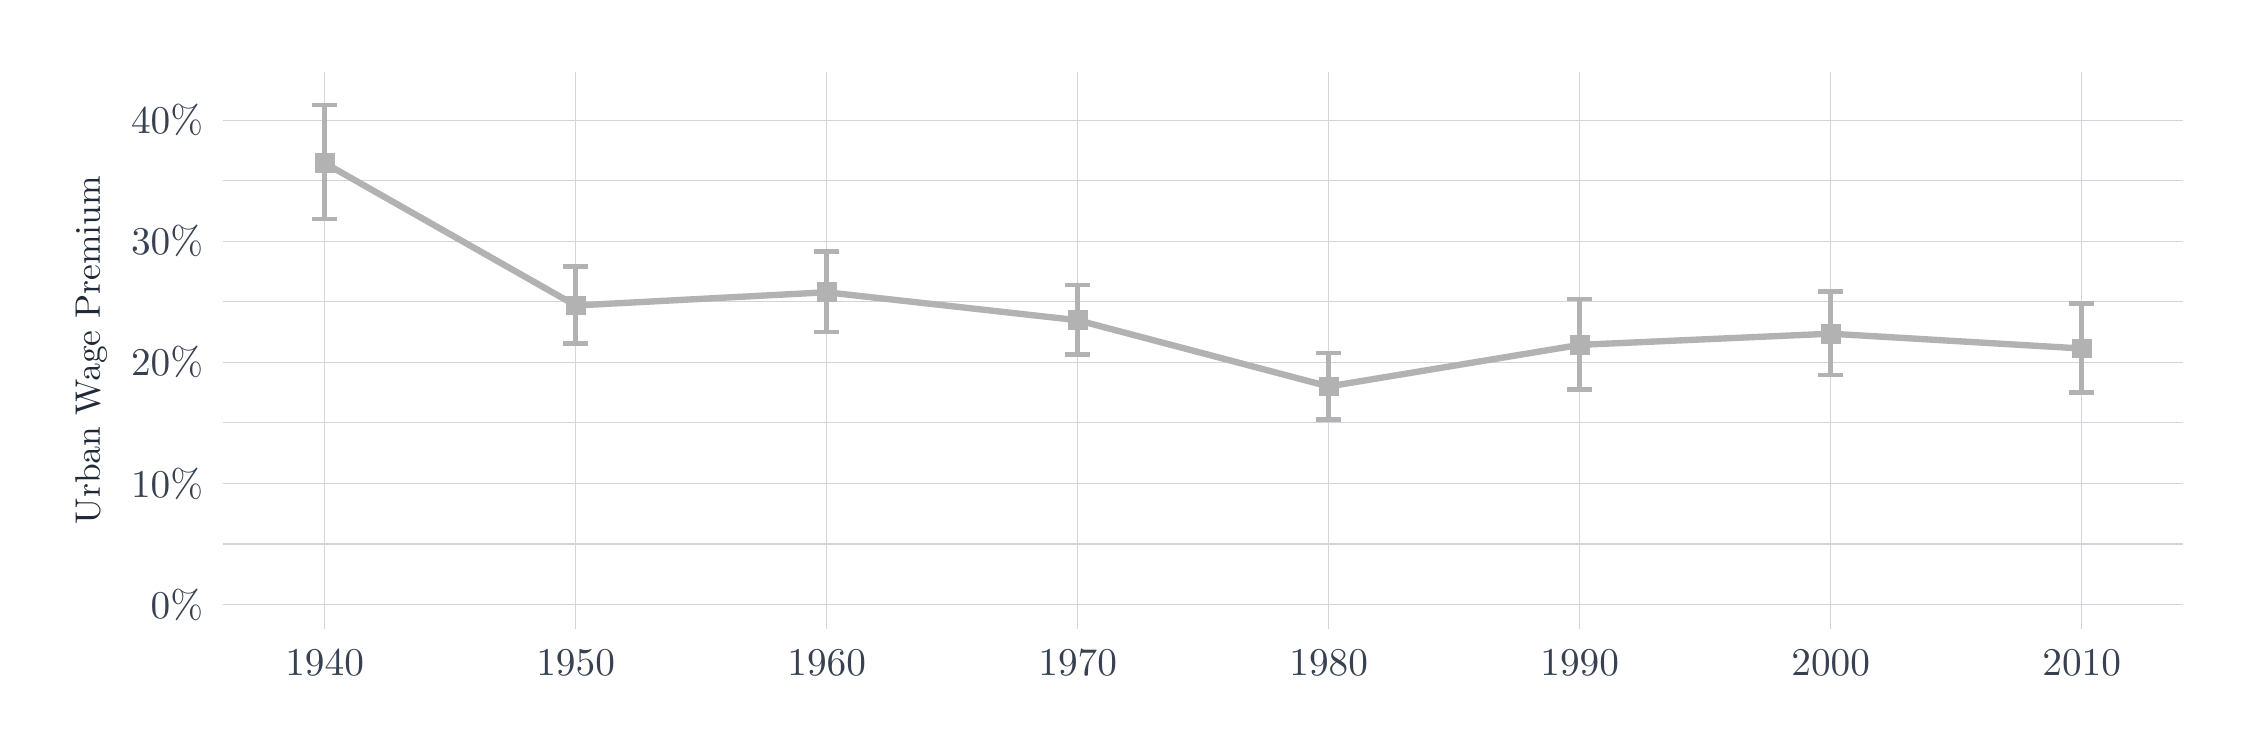
\begin{tikzpicture}[x=1pt,y=1pt]
\definecolor{fillColor}{RGB}{255,255,255}
\path[use as bounding box,fill=fillColor] (0,0) rectangle (794.97,252.94);
\begin{scope}
\path[clip] (  0.00,  0.00) rectangle (794.97,252.94);
\definecolor{drawColor}{RGB}{255,255,255}

\path[draw=drawColor,line width= 0.8pt,line join=round,line cap=round,fill=fillColor] (  0.00,  0.00) rectangle (794.97,252.94);
\end{scope}
\begin{scope}
\path[clip] ( 70.57, 35.76) rectangle (778.97,236.94);
\definecolor{drawColor}{RGB}{255,255,255}
\definecolor{fillColor}{RGB}{255,255,255}

\path[draw=drawColor,line width= 0.8pt,line join=round,line cap=round,fill=fillColor] ( 70.57, 35.76) rectangle (778.97,236.95);
\definecolor{drawColor}{RGB}{209,213,219}

\path[draw=drawColor,line width= 0.4pt,line join=round] ( 70.57, 66.37) --
	(778.97, 66.37);

\path[draw=drawColor,line width= 0.4pt,line join=round] ( 70.57,110.11) --
	(778.97,110.11);

\path[draw=drawColor,line width= 0.4pt,line join=round] ( 70.57,153.85) --
	(778.97,153.85);

\path[draw=drawColor,line width= 0.4pt,line join=round] ( 70.57,197.58) --
	(778.97,197.58);

\path[draw=drawColor,line width= 0.4pt,line join=round] ( 70.57, 44.51) --
	(778.97, 44.51);

\path[draw=drawColor,line width= 0.4pt,line join=round] ( 70.57, 88.24) --
	(778.97, 88.24);

\path[draw=drawColor,line width= 0.4pt,line join=round] ( 70.57,131.98) --
	(778.97,131.98);

\path[draw=drawColor,line width= 0.4pt,line join=round] ( 70.57,175.71) --
	(778.97,175.71);

\path[draw=drawColor,line width= 0.4pt,line join=round] ( 70.57,219.45) --
	(778.97,219.45);

\path[draw=drawColor,line width= 0.4pt,line join=round] (107.30, 35.76) --
	(107.30,236.94);

\path[draw=drawColor,line width= 0.4pt,line join=round] (198.01, 35.76) --
	(198.01,236.94);

\path[draw=drawColor,line width= 0.4pt,line join=round] (288.71, 35.76) --
	(288.71,236.94);

\path[draw=drawColor,line width= 0.4pt,line join=round] (379.42, 35.76) --
	(379.42,236.94);

\path[draw=drawColor,line width= 0.4pt,line join=round] (470.12, 35.76) --
	(470.12,236.94);

\path[draw=drawColor,line width= 0.4pt,line join=round] (560.83, 35.76) --
	(560.83,236.94);

\path[draw=drawColor,line width= 0.4pt,line join=round] (651.53, 35.76) --
	(651.53,236.94);

\path[draw=drawColor,line width= 0.4pt,line join=round] (742.23, 35.76) --
	(742.23,236.94);
\definecolor{drawColor}{gray}{0.70}

\path[draw=drawColor,line width= 2.3pt,line join=round] (107.30,204.04) --
	(198.01,152.55) --
	(288.71,157.33) --
	(379.42,147.22) --
	(470.12,123.29) --
	(560.83,138.32) --
	(651.53,142.36) --
	(742.23,137.00);

\path[draw=drawColor,line width= 1.7pt,line join=round] (102.77,224.97) --
	(111.84,224.97);

\path[draw=drawColor,line width= 1.7pt,line join=round] (107.30,224.97) --
	(107.30,183.83);

\path[draw=drawColor,line width= 1.7pt,line join=round] (102.77,183.83) --
	(111.84,183.83);

\path[draw=drawColor,line width= 1.7pt,line join=round] (193.47,166.69) --
	(202.54,166.69);

\path[draw=drawColor,line width= 1.7pt,line join=round] (198.01,166.69) --
	(198.01,138.75);

\path[draw=drawColor,line width= 1.7pt,line join=round] (193.47,138.75) --
	(202.54,138.75);

\path[draw=drawColor,line width= 1.7pt,line join=round] (284.18,172.04) --
	(293.25,172.04);

\path[draw=drawColor,line width= 1.7pt,line join=round] (288.71,172.04) --
	(288.71,143.00);

\path[draw=drawColor,line width= 1.7pt,line join=round] (284.18,143.00) --
	(293.25,143.00);

\path[draw=drawColor,line width= 1.7pt,line join=round] (374.88,159.93) --
	(383.95,159.93);

\path[draw=drawColor,line width= 1.7pt,line join=round] (379.42,159.93) --
	(379.42,134.79);

\path[draw=drawColor,line width= 1.7pt,line join=round] (374.88,134.79) --
	(383.95,134.79);

\path[draw=drawColor,line width= 1.7pt,line join=round] (465.59,135.40) --
	(474.66,135.40);

\path[draw=drawColor,line width= 1.7pt,line join=round] (470.12,135.40) --
	(470.12,111.46);

\path[draw=drawColor,line width= 1.7pt,line join=round] (465.59,111.46) --
	(474.66,111.46);

\path[draw=drawColor,line width= 1.7pt,line join=round] (556.29,154.89) --
	(565.36,154.89);

\path[draw=drawColor,line width= 1.7pt,line join=round] (560.83,154.89) --
	(560.83,122.26);

\path[draw=drawColor,line width= 1.7pt,line join=round] (556.29,122.26) --
	(565.36,122.26);

\path[draw=drawColor,line width= 1.7pt,line join=round] (646.99,157.67) --
	(656.07,157.67);

\path[draw=drawColor,line width= 1.7pt,line join=round] (651.53,157.67) --
	(651.53,127.47);

\path[draw=drawColor,line width= 1.7pt,line join=round] (646.99,127.47) --
	(656.07,127.47);

\path[draw=drawColor,line width= 1.7pt,line join=round] (737.70,153.34) --
	(746.77,153.34);

\path[draw=drawColor,line width= 1.7pt,line join=round] (742.23,153.34) --
	(742.23,121.15);

\path[draw=drawColor,line width= 1.7pt,line join=round] (737.70,121.15) --
	(746.77,121.15);
\definecolor{fillColor}{gray}{0.70}

\path[fill=fillColor] (103.73,200.48) --
	(110.87,200.48) --
	(110.87,207.61) --
	(103.73,207.61) --
	cycle;

\path[fill=fillColor] (194.44,148.98) --
	(201.58,148.98) --
	(201.58,156.11) --
	(194.44,156.11) --
	cycle;

\path[fill=fillColor] (285.14,153.76) --
	(292.28,153.76) --
	(292.28,160.90) --
	(285.14,160.90) --
	cycle;

\path[fill=fillColor] (375.85,143.65) --
	(382.99,143.65) --
	(382.99,150.78) --
	(375.85,150.78) --
	cycle;

\path[fill=fillColor] (466.55,119.72) --
	(473.69,119.72) --
	(473.69,126.86) --
	(466.55,126.86) --
	cycle;

\path[fill=fillColor] (557.26,134.76) --
	(564.39,134.76) --
	(564.39,141.89) --
	(557.26,141.89) --
	cycle;

\path[fill=fillColor] (647.96,138.79) --
	(655.10,138.79) --
	(655.10,145.93) --
	(647.96,145.93) --
	cycle;

\path[fill=fillColor] (738.67,133.43) --
	(745.80,133.43) --
	(745.80,140.57) --
	(738.67,140.57) --
	cycle;
\end{scope}
\begin{scope}
\path[clip] (  0.00,  0.00) rectangle (794.97,252.94);
\definecolor{drawColor}{RGB}{55,65,81}

\node[text=drawColor,anchor=base east,inner sep=0pt, outer sep=0pt, scale=  1.42] at ( 63.37, 39.61) {0\%};

\node[text=drawColor,anchor=base east,inner sep=0pt, outer sep=0pt, scale=  1.42] at ( 63.37, 83.34) {10\%};

\node[text=drawColor,anchor=base east,inner sep=0pt, outer sep=0pt, scale=  1.42] at ( 63.37,127.08) {20\%};

\node[text=drawColor,anchor=base east,inner sep=0pt, outer sep=0pt, scale=  1.42] at ( 63.37,170.82) {30\%};

\node[text=drawColor,anchor=base east,inner sep=0pt, outer sep=0pt, scale=  1.42] at ( 63.37,214.55) {40\%};
\end{scope}
\begin{scope}
\path[clip] (  0.00,  0.00) rectangle (794.97,252.94);
\definecolor{drawColor}{RGB}{55,65,81}

\node[text=drawColor,anchor=base,inner sep=0pt, outer sep=0pt, scale=  1.42] at (107.30, 18.76) {1940};

\node[text=drawColor,anchor=base,inner sep=0pt, outer sep=0pt, scale=  1.42] at (198.01, 18.76) {1950};

\node[text=drawColor,anchor=base,inner sep=0pt, outer sep=0pt, scale=  1.42] at (288.71, 18.76) {1960};

\node[text=drawColor,anchor=base,inner sep=0pt, outer sep=0pt, scale=  1.42] at (379.42, 18.76) {1970};

\node[text=drawColor,anchor=base,inner sep=0pt, outer sep=0pt, scale=  1.42] at (470.12, 18.76) {1980};

\node[text=drawColor,anchor=base,inner sep=0pt, outer sep=0pt, scale=  1.42] at (560.83, 18.76) {1990};

\node[text=drawColor,anchor=base,inner sep=0pt, outer sep=0pt, scale=  1.42] at (651.53, 18.76) {2000};

\node[text=drawColor,anchor=base,inner sep=0pt, outer sep=0pt, scale=  1.42] at (742.23, 18.76) {2010};
\end{scope}
\begin{scope}
\path[clip] (  0.00,  0.00) rectangle (794.97,252.94);
\definecolor{drawColor}{RGB}{31,41,55}

\node[text=drawColor,rotate= 90.00,anchor=base,inner sep=0pt, outer sep=0pt, scale=  1.28] at ( 26.06,136.35) {Urban Wage Premium};
\end{scope}
\end{tikzpicture}
